\documentclass[tikz, border=5pt]{standalone}

\begin{document}

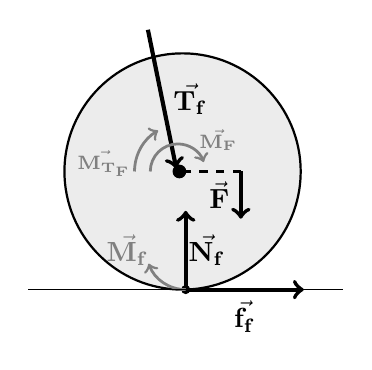
\begin{tikzpicture}

    %% FBD of Front wheel
    % Front wheel
    \draw[thick, fill=gray!15] (-0.04,0) circle(1.5);
    \draw[fill] (-0.08,0) circle(0.08);

    % Normal force
    \draw[->, line width=1.5pt] (0,-1.5) -- (0,-0.5) node[midway,right,xshift=-3] {$\vec{\mathbf{N_f}}$};
    \draw[fill] (0,-1.5) circle(0.05);

    % Applied force on the pedal
    \draw[->, line width=1.5pt] (0.7,0) -- (0.7,-0.6) node[midway,left] {$\vec{\mathbf{F}}$};

    % Frictional force
    \draw[->, line width=1.5pt] (0,-1.5) -- (1.5,-1.5) node[midway,below] {$\vec{\mathbf{f_f}}$};

    % Chassis force
    \draw[->, line width=1.5pt] (-0.48,1.8) -- (-0.08-0.04,0+0.04) node[midway, right] {$\vec{\mathbf{T_f}}$};

    % Moment due to the applied force
    \draw[->, line width=1pt, black!50] (-0.45,0) arc[start angle=180, end angle=20, radius=0.35];
    \node [right, black!50] at (0.05,0.4) {\scriptsize $\vec{\mathbf{M_F}}$};

    % Moment due to the chassis force
    \draw[->, line width=1pt, black!50] (-0.65,0) arc[start angle=180, end angle=120, radius=0.6];
    \node [right, black!50] at (-1.5,0.1) {\scriptsize $\vec{\mathbf{M_{T{_F}}}}$};

    % Moment due to the frictional force
    \draw[->, line width=1pt, black!50] (0,-1.5) arc[start angle=270, end angle=200, radius=0.5];
    \node [left, black!50] at (-0.35,-1) {$\vec{\mathbf{M_f}}$};

    % Pedal
    \draw[thick, dashed] (0.7,0) -- (0,0);

    % Ground
    \draw (-2,-1.5) -- (2,-1.5);

\end{tikzpicture}

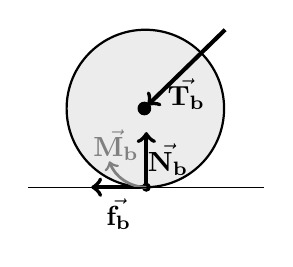
\begin{tikzpicture}

    %% FBD of Back wheel
    % Back wheel
    \draw[thick, fill=gray!15] (-0.0125,0) circle(1);
    \draw[fill] (-0.025,0) circle(0.08);

    % Normal force
    \draw[->, line width=1.5pt] (0,-1) -- (0,-0.3) node[midway, right, xshift=-3.5] {$\vec{\mathbf{N_b}}$};
    \draw[fill] (0,-1) circle(0.05);

    % Frictional force
    \draw[->, line width=1.5pt] (0,-1) -- (-0.7,-1) node[midway,below] {$\vec{\mathbf{f_b}}$};

    % Chassis force
    \draw[->, line width=1.5pt] (1,1) -- (-0.025+0.04,0+0.04) node[midway, below] {$\vec{\mathbf{T_b}}$};

    % Moment due to the frictional force
    \draw[->, line width=1pt, black!50] (0,-1) arc[start angle=270, end angle=200, radius=0.5];
    \node [above, xshift=-1, yshift=6, black!50] at (-0.35,-1) {$\vec{\mathbf{M_b}}$};

    % Ground
    \draw (-1.5,-1) -- (1.5,-1);

\end{tikzpicture}

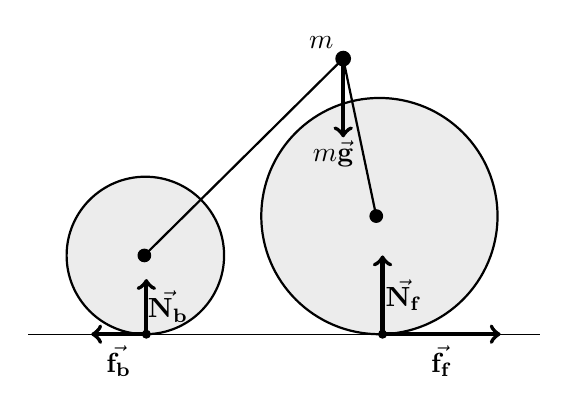
\begin{tikzpicture}

    %% FBD of Entire Bicycle
    \begin{scope}
        % Front wheel
        \draw[thick, fill=gray!15] (-0.04,0) circle(1.5);
        \draw[fill] (-0.08,0) circle(0.08);

        % Normal force
        \draw[->, line width=1.5pt] (0,-1.5) -- (0,-0.5) node[midway,right,xshift=-3] {$\vec{\mathbf{N_f}}$};
        \draw[fill] (0,-1.5) circle(0.05);

        % Frictional force
        \draw[->, line width=1.5pt] (0,-1.5) -- (1.5,-1.5) node[midway,below] {$\vec{\mathbf{f_f}}$};
    \end{scope}
    \begin{scope}[xshift=-3cm, yshift=-0.5cm]
        % Back wheel
        \draw[thick, fill=gray!15] (-0.0125,0) circle(1);
        \draw[fill] (-0.025,0) circle(0.08);

        % Normal force
        \draw[->, line width=1.5pt] (0,-1) -- (0,-0.3) node[midway, right, xshift=-3.5] {$\vec{\mathbf{N_b}}$};
        \draw[fill] (0,-1) circle(0.05);

        % Frictional force
        \draw[->, line width=1.5pt] (0,-1) -- (-0.7,-1) node[midway,below] {$\vec{\mathbf{f_b}}$};
    \end{scope}

    % Ground
    \draw (-4.5,-1.5) -- (2,-1.5);

    % Chassis
    \draw[thick] (-0.08,0) -- (-0.5,2);
    \draw[thick] (-0.5,2) -- (-3.025,-0.5);

    % Rider
    \fill (-0.5,2) circle(0.1);
    \node [left] at (-0.5,2.2) {\(m\)};

    % Weight of rider
    \draw[->, line width=1.5pt] (-0.5,2) -- (-0.5,1) node[right, xshift=-15pt, yshift=-6pt] {\(m\vec{\mathbf{g}}\)};

\end{tikzpicture}

\end{document}
